% Options for packages loaded elsewhere
\PassOptionsToPackage{unicode}{hyperref}
\PassOptionsToPackage{hyphens}{url}
\PassOptionsToPackage{dvipsnames,svgnames,x11names}{xcolor}
%
\documentclass[
  letterpaper,
  DIV=11,
  numbers=noendperiod]{scrartcl}

\usepackage{amsmath,amssymb}
\usepackage{iftex}
\ifPDFTeX
  \usepackage[T1]{fontenc}
  \usepackage[utf8]{inputenc}
  \usepackage{textcomp} % provide euro and other symbols
\else % if luatex or xetex
  \usepackage{unicode-math}
  \defaultfontfeatures{Scale=MatchLowercase}
  \defaultfontfeatures[\rmfamily]{Ligatures=TeX,Scale=1}
\fi
\usepackage{lmodern}
\ifPDFTeX\else  
    % xetex/luatex font selection
\fi
% Use upquote if available, for straight quotes in verbatim environments
\IfFileExists{upquote.sty}{\usepackage{upquote}}{}
\IfFileExists{microtype.sty}{% use microtype if available
  \usepackage[]{microtype}
  \UseMicrotypeSet[protrusion]{basicmath} % disable protrusion for tt fonts
}{}
\makeatletter
\@ifundefined{KOMAClassName}{% if non-KOMA class
  \IfFileExists{parskip.sty}{%
    \usepackage{parskip}
  }{% else
    \setlength{\parindent}{0pt}
    \setlength{\parskip}{6pt plus 2pt minus 1pt}}
}{% if KOMA class
  \KOMAoptions{parskip=half}}
\makeatother
\usepackage{xcolor}
\setlength{\emergencystretch}{3em} % prevent overfull lines
\setcounter{secnumdepth}{-\maxdimen} % remove section numbering
% Make \paragraph and \subparagraph free-standing
\makeatletter
\ifx\paragraph\undefined\else
  \let\oldparagraph\paragraph
  \renewcommand{\paragraph}{
    \@ifstar
      \xxxParagraphStar
      \xxxParagraphNoStar
  }
  \newcommand{\xxxParagraphStar}[1]{\oldparagraph*{#1}\mbox{}}
  \newcommand{\xxxParagraphNoStar}[1]{\oldparagraph{#1}\mbox{}}
\fi
\ifx\subparagraph\undefined\else
  \let\oldsubparagraph\subparagraph
  \renewcommand{\subparagraph}{
    \@ifstar
      \xxxSubParagraphStar
      \xxxSubParagraphNoStar
  }
  \newcommand{\xxxSubParagraphStar}[1]{\oldsubparagraph*{#1}\mbox{}}
  \newcommand{\xxxSubParagraphNoStar}[1]{\oldsubparagraph{#1}\mbox{}}
\fi
\makeatother


\providecommand{\tightlist}{%
  \setlength{\itemsep}{0pt}\setlength{\parskip}{0pt}}\usepackage{longtable,booktabs,array}
\usepackage{calc} % for calculating minipage widths
% Correct order of tables after \paragraph or \subparagraph
\usepackage{etoolbox}
\makeatletter
\patchcmd\longtable{\par}{\if@noskipsec\mbox{}\fi\par}{}{}
\makeatother
% Allow footnotes in longtable head/foot
\IfFileExists{footnotehyper.sty}{\usepackage{footnotehyper}}{\usepackage{footnote}}
\makesavenoteenv{longtable}
\usepackage{graphicx}
\makeatletter
\newsavebox\pandoc@box
\newcommand*\pandocbounded[1]{% scales image to fit in text height/width
  \sbox\pandoc@box{#1}%
  \Gscale@div\@tempa{\textheight}{\dimexpr\ht\pandoc@box+\dp\pandoc@box\relax}%
  \Gscale@div\@tempb{\linewidth}{\wd\pandoc@box}%
  \ifdim\@tempb\p@<\@tempa\p@\let\@tempa\@tempb\fi% select the smaller of both
  \ifdim\@tempa\p@<\p@\scalebox{\@tempa}{\usebox\pandoc@box}%
  \else\usebox{\pandoc@box}%
  \fi%
}
% Set default figure placement to htbp
\def\fps@figure{htbp}
\makeatother

\KOMAoption{captions}{tableheading}
\makeatletter
\@ifpackageloaded{caption}{}{\usepackage{caption}}
\AtBeginDocument{%
\ifdefined\contentsname
  \renewcommand*\contentsname{Table of contents}
\else
  \newcommand\contentsname{Table of contents}
\fi
\ifdefined\listfigurename
  \renewcommand*\listfigurename{List of Figures}
\else
  \newcommand\listfigurename{List of Figures}
\fi
\ifdefined\listtablename
  \renewcommand*\listtablename{List of Tables}
\else
  \newcommand\listtablename{List of Tables}
\fi
\ifdefined\figurename
  \renewcommand*\figurename{Figure}
\else
  \newcommand\figurename{Figure}
\fi
\ifdefined\tablename
  \renewcommand*\tablename{Table}
\else
  \newcommand\tablename{Table}
\fi
}
\@ifpackageloaded{float}{}{\usepackage{float}}
\floatstyle{ruled}
\@ifundefined{c@chapter}{\newfloat{codelisting}{h}{lop}}{\newfloat{codelisting}{h}{lop}[chapter]}
\floatname{codelisting}{Listing}
\newcommand*\listoflistings{\listof{codelisting}{List of Listings}}
\makeatother
\makeatletter
\makeatother
\makeatletter
\@ifpackageloaded{caption}{}{\usepackage{caption}}
\@ifpackageloaded{subcaption}{}{\usepackage{subcaption}}
\makeatother

\usepackage{bookmark}

\IfFileExists{xurl.sty}{\usepackage{xurl}}{} % add URL line breaks if available
\urlstyle{same} % disable monospaced font for URLs
\hypersetup{
  pdftitle={EPIB 629: Knowledge Synthesis},
  pdfauthor={James (Jay) Brophy},
  colorlinks=true,
  linkcolor={blue},
  filecolor={Maroon},
  citecolor={Blue},
  urlcolor={Blue},
  pdfcreator={LaTeX via pandoc}}


\title{EPIB 629: Knowledge Synthesis}
\usepackage{etoolbox}
\makeatletter
\providecommand{\subtitle}[1]{% add subtitle to \maketitle
  \apptocmd{\@title}{\par {\large #1 \par}}{}{}
}
\makeatother
\subtitle{Fall 2025}
\author{James (Jay) Brophy}
\date{2025-09-02}

\begin{document}
\maketitle


\href{}{{[}PDF version{]}}

\begin{longtable}[]{@{}
  >{\raggedright\arraybackslash}p{(\linewidth - 2\tabcolsep) * \real{0.4500}}
  >{\raggedright\arraybackslash}p{(\linewidth - 2\tabcolsep) * \real{0.5500}}@{}}
\toprule\noalign{}
\begin{minipage}[b]{\linewidth}\raggedright
\textbf{About me}
\end{minipage} & \begin{minipage}[b]{\linewidth}\raggedright
\textbf{About class}
\end{minipage} \\
\midrule\noalign{}
\endhead
\bottomrule\noalign{}
\endlastfoot
\href{https://brophyj.com}{james brophy} & \\
james.brophy@mcgill.ca &
\href{https://mycourses2.mcgill.ca/d2l/home/770484}{mycourses2.mcgill.ca} \\
Location: & 2001 McGill College Avenue \textbf{Room 464} \\
Hours: immediately after class or email me to schedule another time &
Hours: Tuesday/Thursday 8:35h-9:55h \\
Office: Homeless (visiting faculty area) & \\
\end{longtable}

\section{Course Description}\label{course-description}

EPIB 629 is a graduate level course providing a detailed description of
the systematic review process, discusses the strengths and limitations
of the method, including a step-by-step guidance on how to perform a
systematic review, and how to critically appraise systematic reviews.
Specific topics to be covered include: formulation of the review
question, searching of literature, quality assessment of studies, data
extraction, meta-analytic methods, and report writing. The course will
extensively cover statistical issues of meta-analysis.

\section{Eligibility}\label{eligibility}

Introductory level training in epidemiology (e.g.~EPIB 601) and
biostatistics (e.g.~EPIB 607). Specifically required is some basic
familiarity with statistical coding, ideally \texttt{R} but
\texttt{Python} is also acceptable (although the \texttt{Python} support
I can provide is more limited). All others must seek the instructor's
permission.

\section{Course Format}\label{course-format}

This course will be taught predominately with in-person sessions. Rarely
sessions may be delivered remotely via zoom if a guest lecturer from an
outside institution is invited. Every effort will be made to provide a
supportive learning environment throughout this course. While the course
has been designed to maximize learning via in-person learning approach,
further modifications may be required as we work our way through the
semester so understanding and flexibility are important.
\href{https://www.mcgill.ca/tls/students}{McGill's Teaching and Learning
Services} offer numerous student learning resources.

Students should regularly check MyCourses for announcements, content,
and other course related communication (i.e., at least twice per week).
I recommend that students enable MyCourses'
\href{https://mcgill.service-now.com/itportal?id=kb_article&sysparm_article=KB001108}{notification
feature}.

\section{Learning Outcomes}\label{learning-outcomes}

By the end of this course, students will be able to:~\\
• Explain the rationale for conducting a systematic review and/or
meta-analysis~\\
• Understand the role of systematic reviews and meta-analyses in the
practice of evidence-based medicine and public health~\\
• Describe the key components of a systematic review and
meta-analysis~\\
• Critically appraise published systematic reviews and meta-analyses~\\
• Develop a protocol for a knowledge synthesis study, applying the
knowledge and concepts discussed in this course~\\
• Conduct a knowledge synthesis study~

\section{Course Content}\label{course-content}

Knowledge synthesis is critical for evidence-based clinical and public
health practice. The widespread and growing application of systematic
reviews and meta-analyses to key research and clinical questions makes
it essential for that all health professionals can critically assess
this research design and for research producers be able to conduct their
own reviews. This course will provide a detailed description of the
systematic review process, discuss its strengths and limitations,
provide step-by-step guidance on how its performance, and how to
critically appraise them. Specific topics to be covered include:
formulation of the review question, searching of literature, quality
assessment of studies, data extraction, meta-analytic methods, and
report writing. The course will rely heavily on statistical methods that
enable the synthesis of the available evidence. Statistical issues such
as statistical model selection including problem sets with practical
examples of fixed and random effects models, as well as examples of
methods to evaluate heterogeneity, individual patient level data,
network meta-analysis and graphical and tabular data presentations will
form a large part of the course.~

Although each class session is 1.5 hours, there will inevitably be
topics that come up that we can't fully address in class. I encourage
you to use the
\href{https://mycourses2.mcgill.ca/d2l/le/631790/discussions/List}{Discussion}
section of MyCourses to post questions or comments there. I may also
post any additional pertinent links to additional readings for those
interested.~

Students will be required to complete a systematic review on the topic
of their choosing during the course. The goal is to consolidate the
knowledge and experiences gained during this class to complete a
knowledge synthesis study that can be subsequently submitted for
peer-review publication.~

\section{Course materials}\label{course-materials}

Given the important role that systematic reviews (SR) and meta-analyses
play in healthcare research and practice, it is not suprising that many
different resources are available. The McGill library has over 100
titles with systematic reviews in the title and the number on PubMed is
literally uncountable. ~

The Cochrane Handbook for Systematic Reviews of Interventions is the
most widely used reference for systematic reviews and meta-analyses. The
6th edition (2019) is available online at
\href{https://training.cochrane.org/handbook/current}{Cochrane
Handbook}. The Cochrane Handbook is a comprehensive resource that covers
all aspects of conducting systematic reviews and meta-analyses,
including study design, data analysis, and reporting. It is an essential
reference for anyone involved in conducting or interpreting systematic
reviews and meta-analyses.~

Other useful Cochrane resouces can be found
\href{https://training.cochrane.org/resources}{here}.~~

For selected topics, this course will follow these two texts~

\textbf{Systematic Reviews in Health ResearchMeta-Analysis in Context}
(3rd edition 2022) edited by M Egger, JPT Higgins, and G Davey Smith.
The text is
\href{https://onlinelibrary-wiley-com.proxy3.library.mcgill.ca/doi/book/10.1002/9781119099369}{available
online at the McGill library} ~~\\
\textbf{Systematic Reviews to Support Evidence-Based Medicine How to
appraise, conduct and publish reviews}(3rd Edition 2022) KS Khan, Javier
Zamora. The text is
\href{https://www-taylorfrancis-com.proxy3.library.mcgill.ca/books/edit/10.1201/9781003220039/systematic-reviews-support-evidence-based-medicine-khalid-saeed-khan-javier-zamora}{available
online at the McGill library} ~~

Bayesian meta-analysis is not really covered in this reference textbook.
Fortunately new textbook \textbf{Bayesian Meta-Analysis: a practical
introduction} by Robert Grant \& Gian Luca di Tanna should be available
by the fall 2025.~~

As no one textbook can cover all aspects of SR/MA that we will be
exploring, we will also read specific published articles that will be
posted on MyCourses.

\section{Computing language}\label{computing-language}

The computing language of choice for the course is \texttt{R}. There are
several reasons for this choice including its open source and rich
online community which means help is often only a Google away. R has
become the \emph{lingua franca} for much of the
epidemiology/biostatistical universe. Currently, the
\href{https://cran.r-project.org}{CRAN package repository} features
22087 R packages including over 60 dedicated to meta-analysis. The most
popular packages are \texttt{meta}, \texttt{metafor}, \texttt{metagear},
\texttt{dmetar}, and \texttt{netmeta} for network metanalysis. Bayesian
meta-analysis can be performed with the following packages
\texttt{bayesmeta}, \texttt{RoBMA} and \texttt{brms}. ~

Of course, other languages such as Python can be used but the support I
can provide is more limited. Stata is a popular software, but I see no
reason to support a proprietary software when excellent open source
options exist. Also I consider the scripting and reproducibility offered
by R-Markdown / Quarto / Jupyter notebooks provides additional
advantages for choosing \texttt{R} or \texttt{Python}.~

\href{https://link-springer-com.proxy3.library.mcgill.ca/book/10.1007/978-3-319-21416-0}{Meta-analysis
with R} provides a comprehensive introduction to performing
meta-analysis using the statistical software R and is available from the
McGill library.

\section{Evaluation}\label{evaluation}

\begin{longtable}[]{@{}
  >{\raggedright\arraybackslash}p{(\linewidth - 4\tabcolsep) * \real{0.3333}}
  >{\raggedright\arraybackslash}p{(\linewidth - 4\tabcolsep) * \real{0.3333}}
  >{\raggedright\arraybackslash}p{(\linewidth - 4\tabcolsep) * \real{0.3333}}@{}}
\toprule\noalign{}
\begin{minipage}[b]{\linewidth}\raggedright
Name of Assignment
\end{minipage} & \begin{minipage}[b]{\linewidth}\raggedright
Date
\end{minipage} & \begin{minipage}[b]{\linewidth}\raggedright
\% of Final Grade
\end{minipage} \\
\midrule\noalign{}
\endhead
\bottomrule\noalign{}
\endlastfoot
In class participation & ongoing & 10\% \\
Critical appraisal of selected published article (750 word limit) & see
schedule & 20\% \\
Development of a new knowledge synthesis protocol (750 word limit) & see
schedule & 20\% \\
In class quiz (30 minute) & & 25\% \\
Final protocol oral presentation with results (3MT format) & & 25\% \\
\end{longtable}

{In class participation:} \textbf{Active} participation means showing up
for each class \emph{having read and engaged with any material
assigned}, focusing during class discussion and being intellectually
engaged;~

{Critical appraisal:} Each student will choose a published SR /MA that
they will critique with a maximum 750 word essay ~

{Development of knowledge synthesis protocol:} Students are required to
submit a written outline (maximum 750 words) of a SR/MA protocol of
their own choosing . This submission should include
background/rationale, the objective of the study, the methods, expected
outcome. More details can be found by following the PRISMA checklist
which should be included as an appendix (doesn't count toward word
limit)~

{Final oral presentation:} Students will have 3 minutes or less and a
single static slide to communicate their research! There will then be 5
minutes to respond to questions from the audience. (see details
\href{https://www.mcgill.ca/involvement/channels/event/3mt-mt180-competition-2024-353339}{here})

\begin{figure}[H]

{\centering \pandocbounded{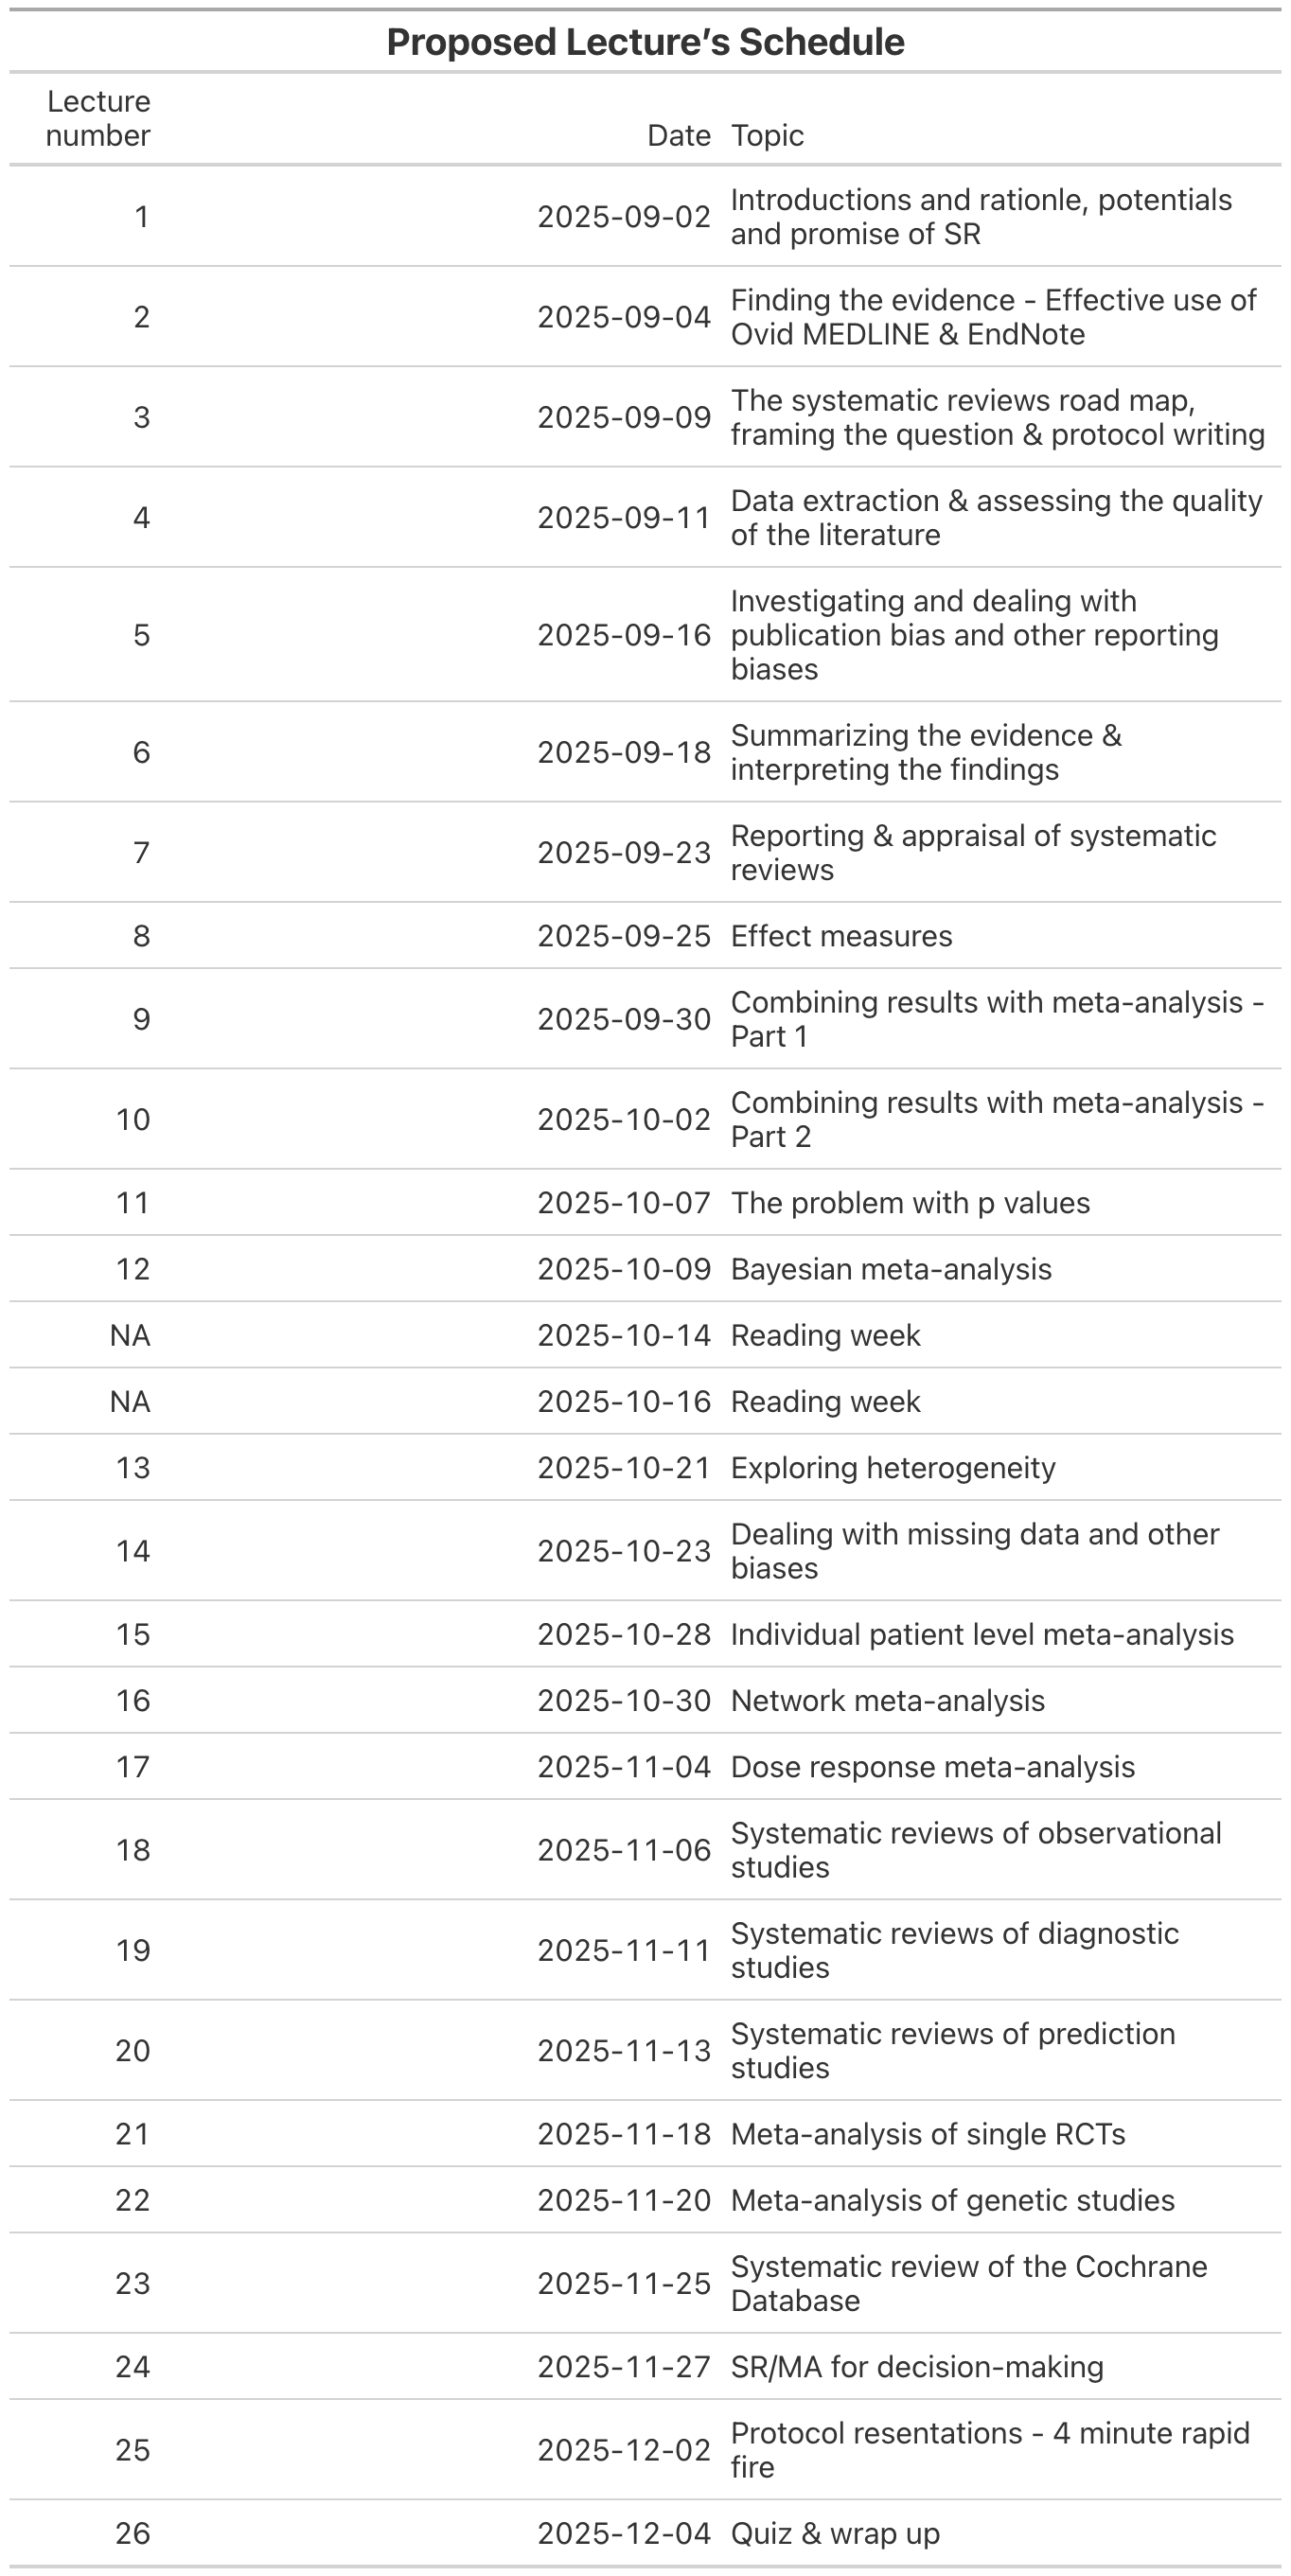
\includegraphics[keepaspectratio]{schedule.png}}

}

\caption{Proposed Lecture's Schedule}

\end{figure}%

\section{Academic Integrity}\label{academic-integrity}

The Department of Epidemiology and Biostatistics has asked instructors
to remind students of McGill University regulations regarding academic
integrity and plagiarism. These are excerpted below.

\section{Academic offences}\label{academic-offences}

The integrity of University academic life and of the degrees the
University confers is dependent upon the honesty and soundness of the
teacher- student learning relationship and, as well, that of the
evaluation process. Conduct by any member of the University community
that adversely affects this relationship or this process must,
therefore, be considered a serious offence. McGill University values
academic integrity. Therefore all students must understand the meaning
and consequences of cheating, plagiarism and other academic offences
under the Code of Student Conduct and Disciplinary Procedures (see
http://www.mcgill.ca/integrity for more information).

L'université McGill attache une haute importance à l'honnêteté
académique. Il incombe par conséquent à tous les étudiants de comprendre
ce que l'on entend par tricherie, plagiat et autres infractions
académiques, ainsi que les conséquences que peuvent avoir de telles
actions, selon le Code de conduite de l'étudiant et des procédures
disciplinaires (pour de plus amples renseignements, veuillez consulter
le site http://www.mcgill.ca/integrity).

\subsection{Plagiarism}\label{plagiarism}

\begin{itemize}
\tightlist
\item
  \textbf{(a)} No student shall, with intent to deceive, represent the
  work of another person as their own in any academic writing or
  assignment.
\item
  \textbf{(b)} If a student submits another's work, it will be presumed
  they intended to deceive unless proven otherwise.
\item
  \textbf{(c)} No student shall contribute work to another student
  knowing it may be submitted as their own.
\end{itemize}

\subsection{Cheating -- No student
shall}\label{cheating-no-student-shall}

\begin{itemize}
\tightlist
\item
  \textbf{(a)} In the course of an examination, obtain or attempt to
  obtain information from another student or unauthorized source, or
  give/attempt to give information to another student.
\item
  \textbf{(b)} Represent or attempt to represent oneself as another or
  have oneself represented by another in an examination or paper
  preparation.
\item
  \textbf{(c)} Submit, without approval, any academic writing or project
  that has been or is being submitted elsewhere.
\item
  \textbf{(d)} Submit work containing a known false statement or
  fabricated reference.
\end{itemize}

Downloaded and excerpted from A Handbook on Student Rights and
Responsibilities, 2010. Available on-line at
http://www.mcgill.ca/students/srr/academicrights/integrity/cheating

\section{Language Rights}\label{language-rights}

``In accord with McGill University's Charter of Students' Rights,
students in this course have the right to submit in English or in French
any written work that is to be graded. This does not apply to courses in
which acquiring proficiency in a language is one of the objectives.''

« Conformément à la Charte des droits de l'étudiant de l'Université
McGill, chaque étudiant a le droit de soumettre en français ou en
anglais tout travail écrit devant être noté (sauf dans le cas des cours
dont l'un des objets est la maîtrise d'une langue). »




\end{document}
